Nous avons ainsi étudié trois types d'échantillons différents :\\
\begin{itemize}
    \item Le brut, monocristallin, en sortie de fonderie
    \item L'alliage après remise en solution (premier traitement thermique)
    \item L'alliage en fin de traitement, après les deux revenus.\\\\
\end{itemize}



Nous devons donc étudier leur microstructure pour déterminer l'influence des 
différents traitements thermiques sur l'alliage, étant donné que cette microstructure
est le paramètre clé qui va déterminer les propriétés mécaniques de l'alliage,
et notamment sa résistance au fluage.

\subsection*{Brut de fonderie}

Étudions tout d'abord les propriétés du brut après fonderie.\\\\


% \centerline{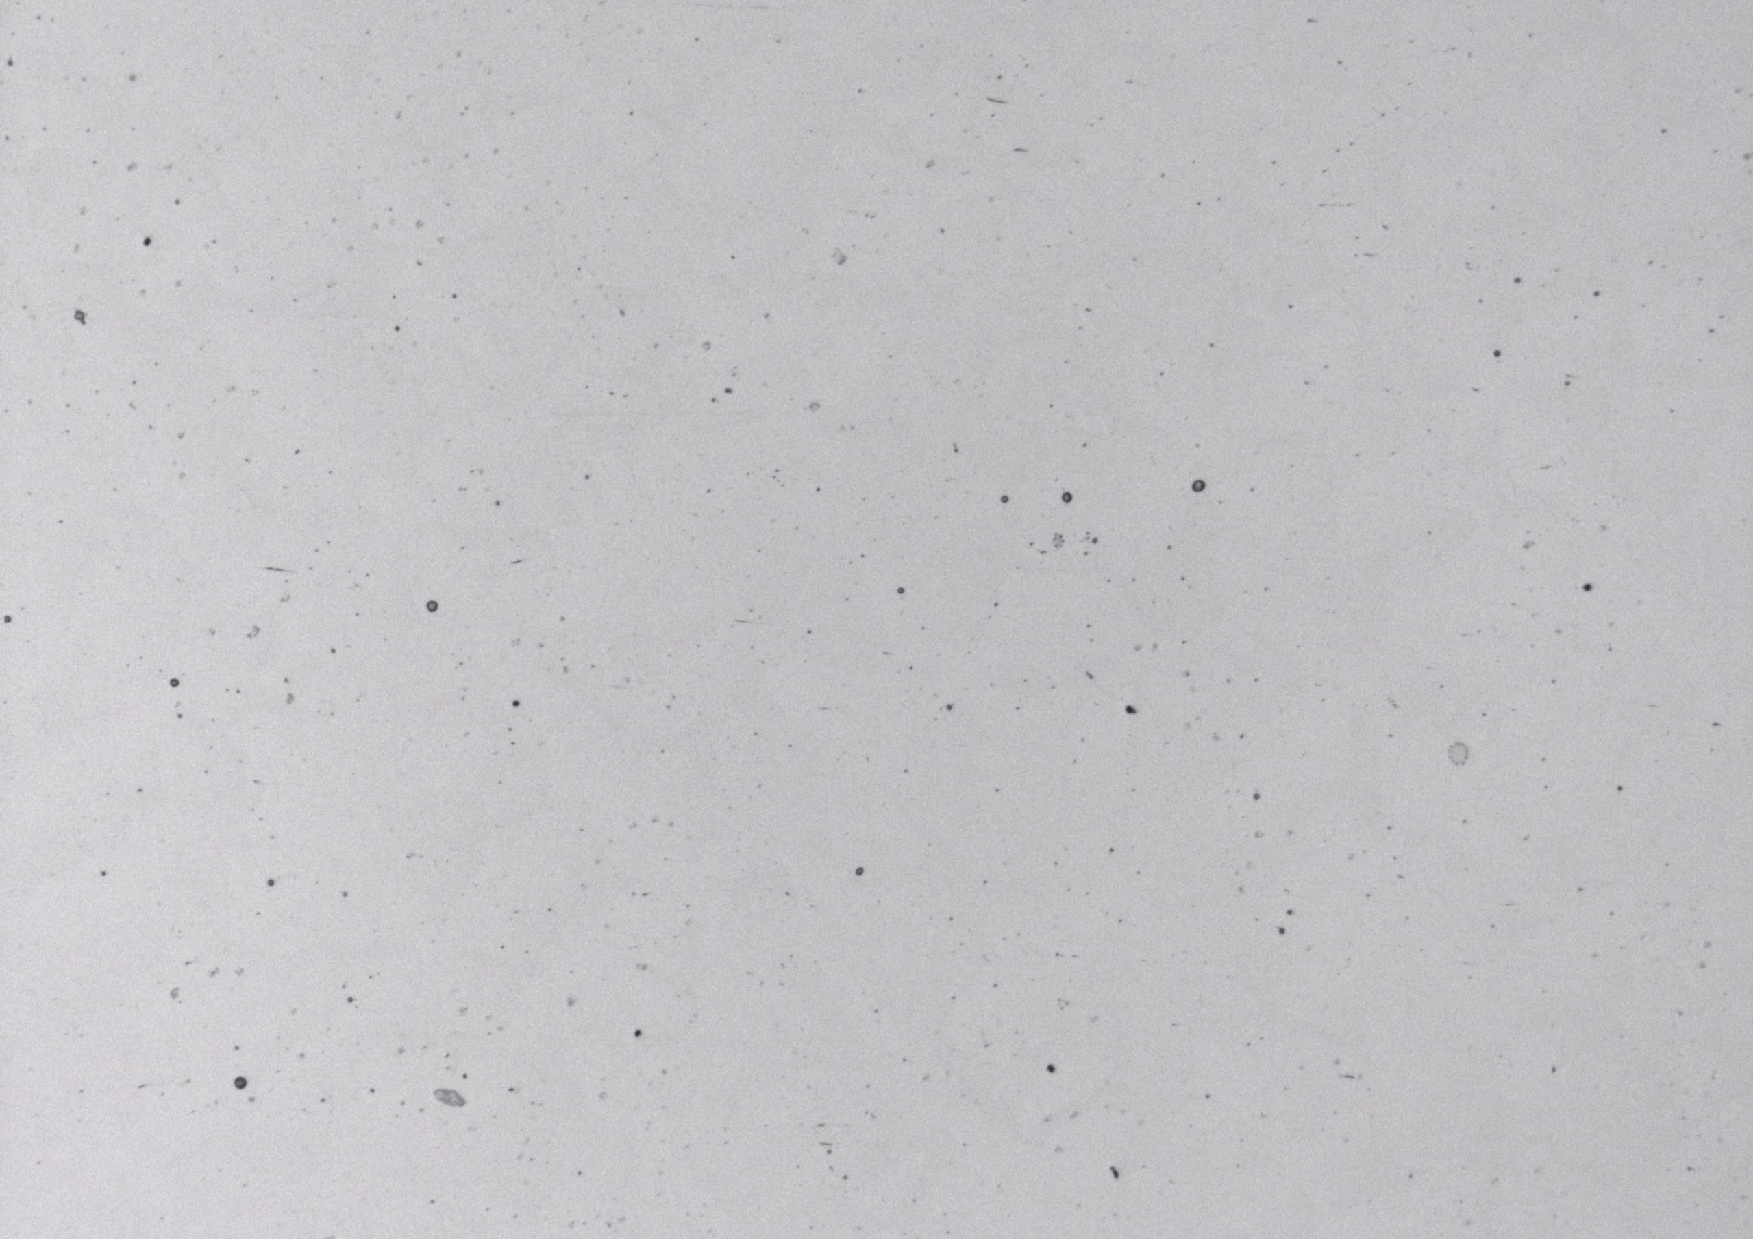
\includegraphics[width=0.75\textwidth]{images_optique/brut.pdf}}
% \legend{Le brut de fonderie vu au microscope optique}

\begin{figure}[htbp]
    \centering
    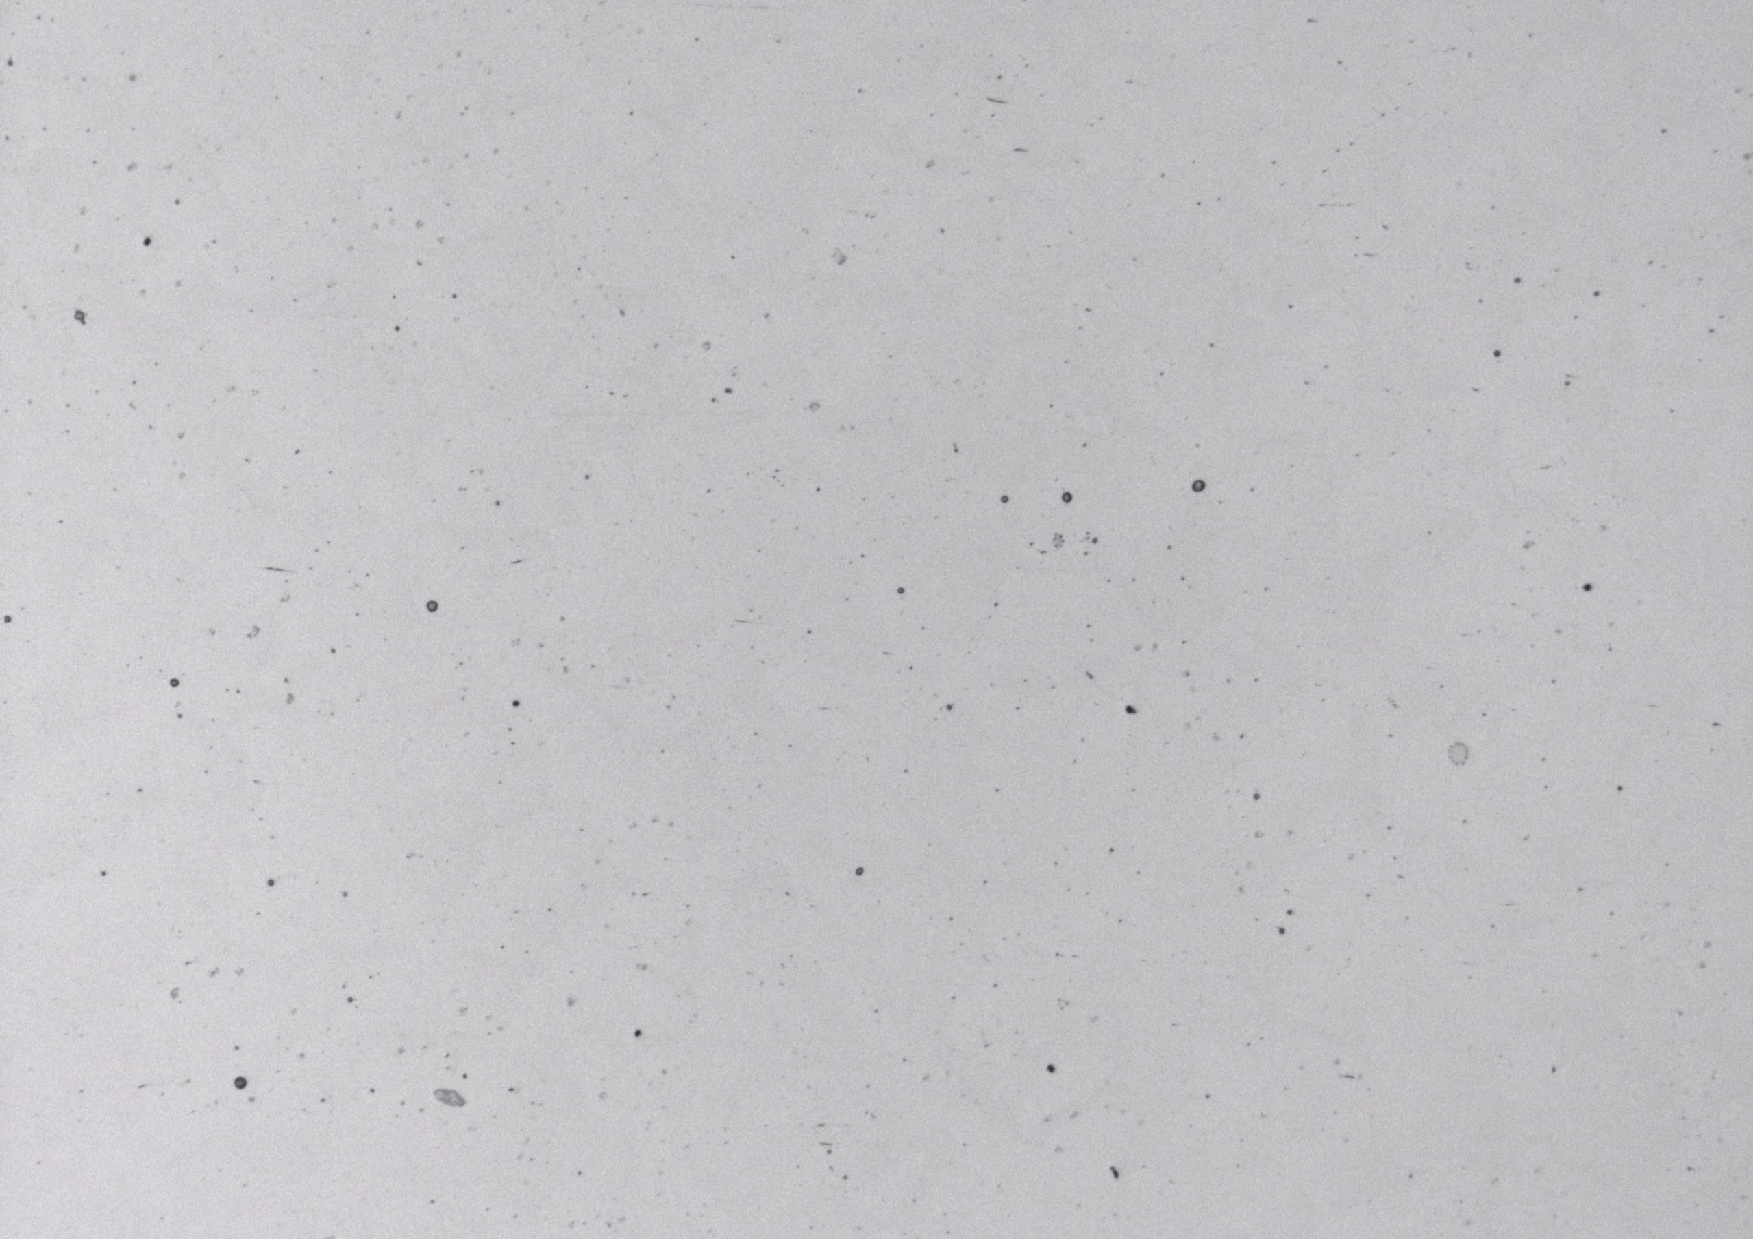
\includegraphics[width=0.75\textwidth]{images_optique/brut.pdf}
    \caption{Echantillon brut de fonderie vu au microscope optique}
    \label{}
\end{figure}


Vu au microscope optique, sa surface (après polissage) est lisse
et présente peu de défauts. Cependant, la surface possède 
également de petites tâches noires : ces tâches sont des \emph{pores},
c'est à dire des trous à la surface de l'échantillon. Il y a à ces endroits 
des lacunes importantes dans la maille cristalline, et il manque donc 
une petite portion du matériau. Nous observons également de plus 
petites tâches grises : il s'agit d'agrégats eutectiques, formés lors du refroidissement du liquide.


% \centerline{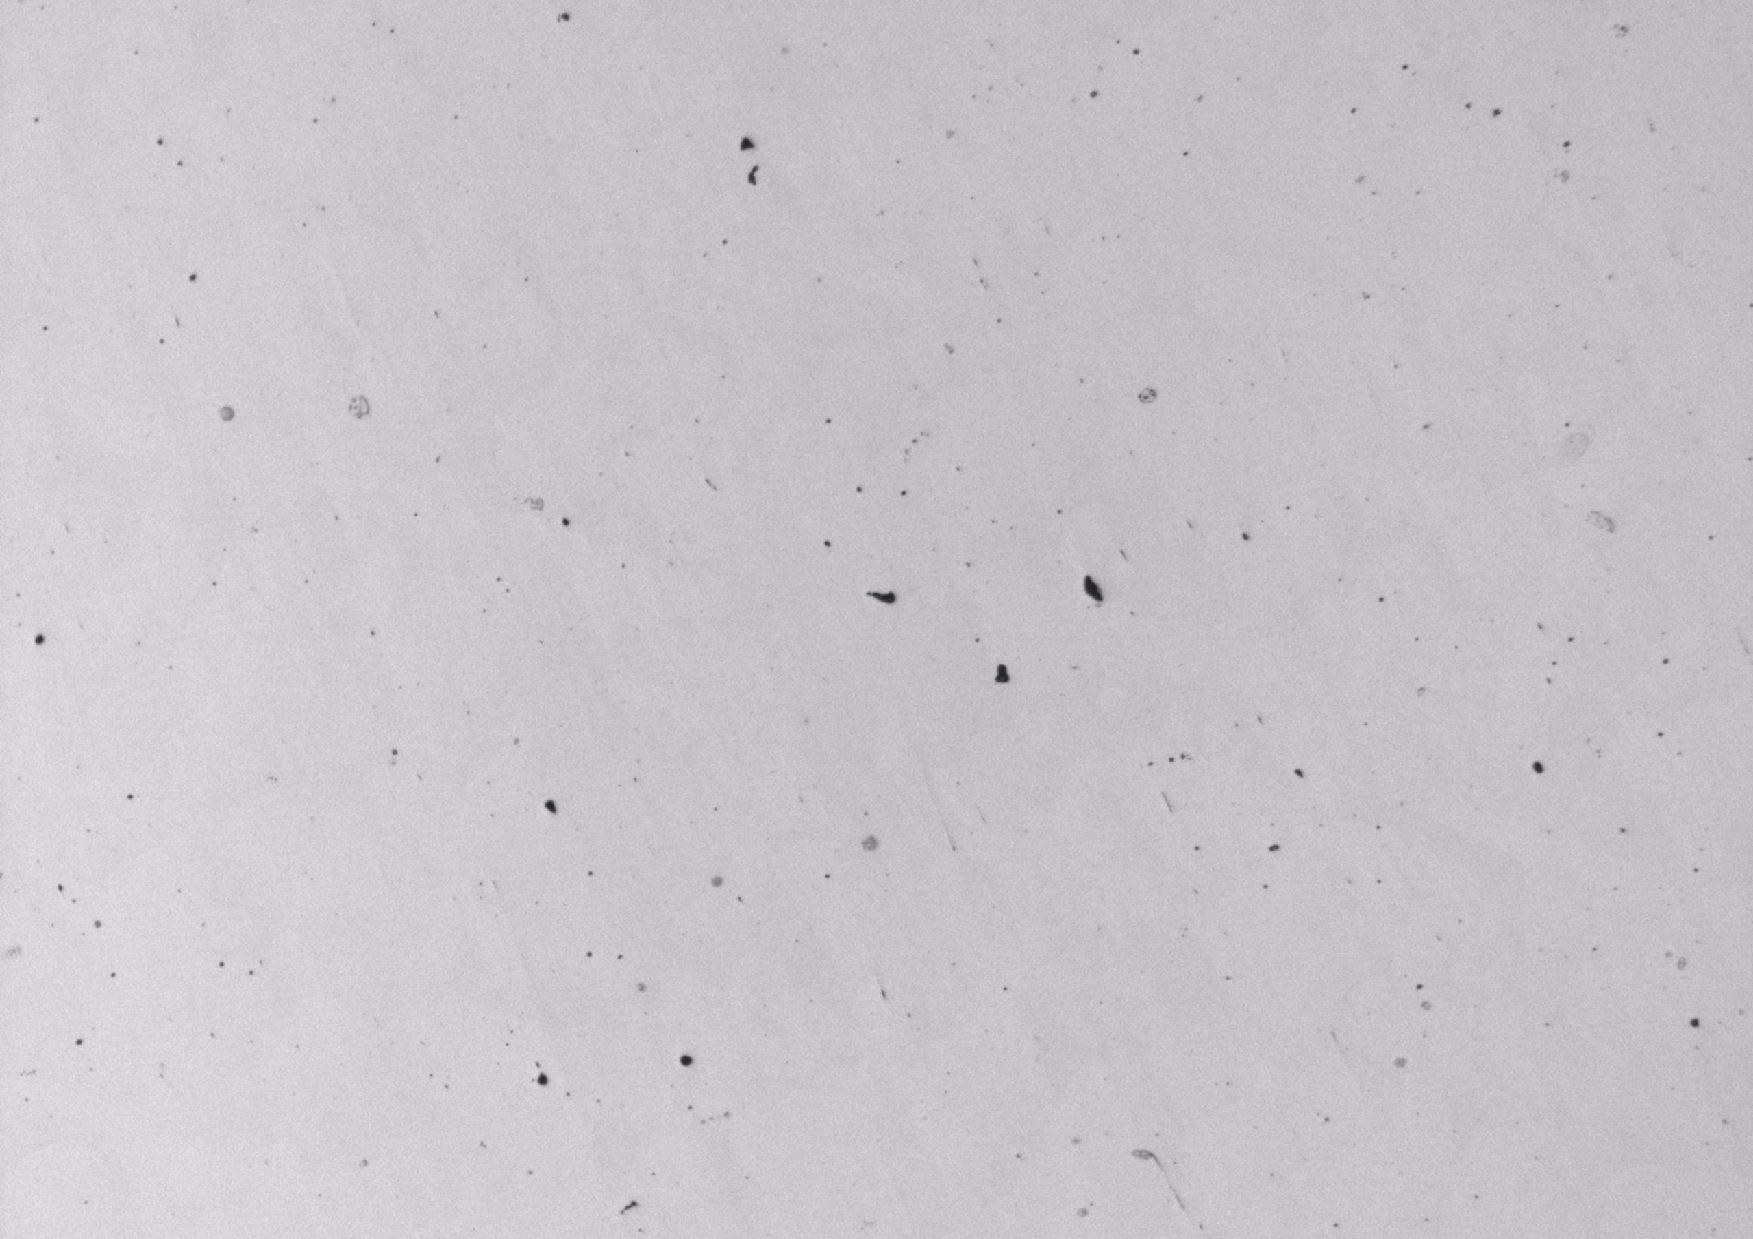
\includegraphics[width=0.75\textwidth]{images_optique/brut2.pdf}}
% \legend{Le brut de fonderie vu au microscope optique}

\begin{figure}[htbp]
    \centering
    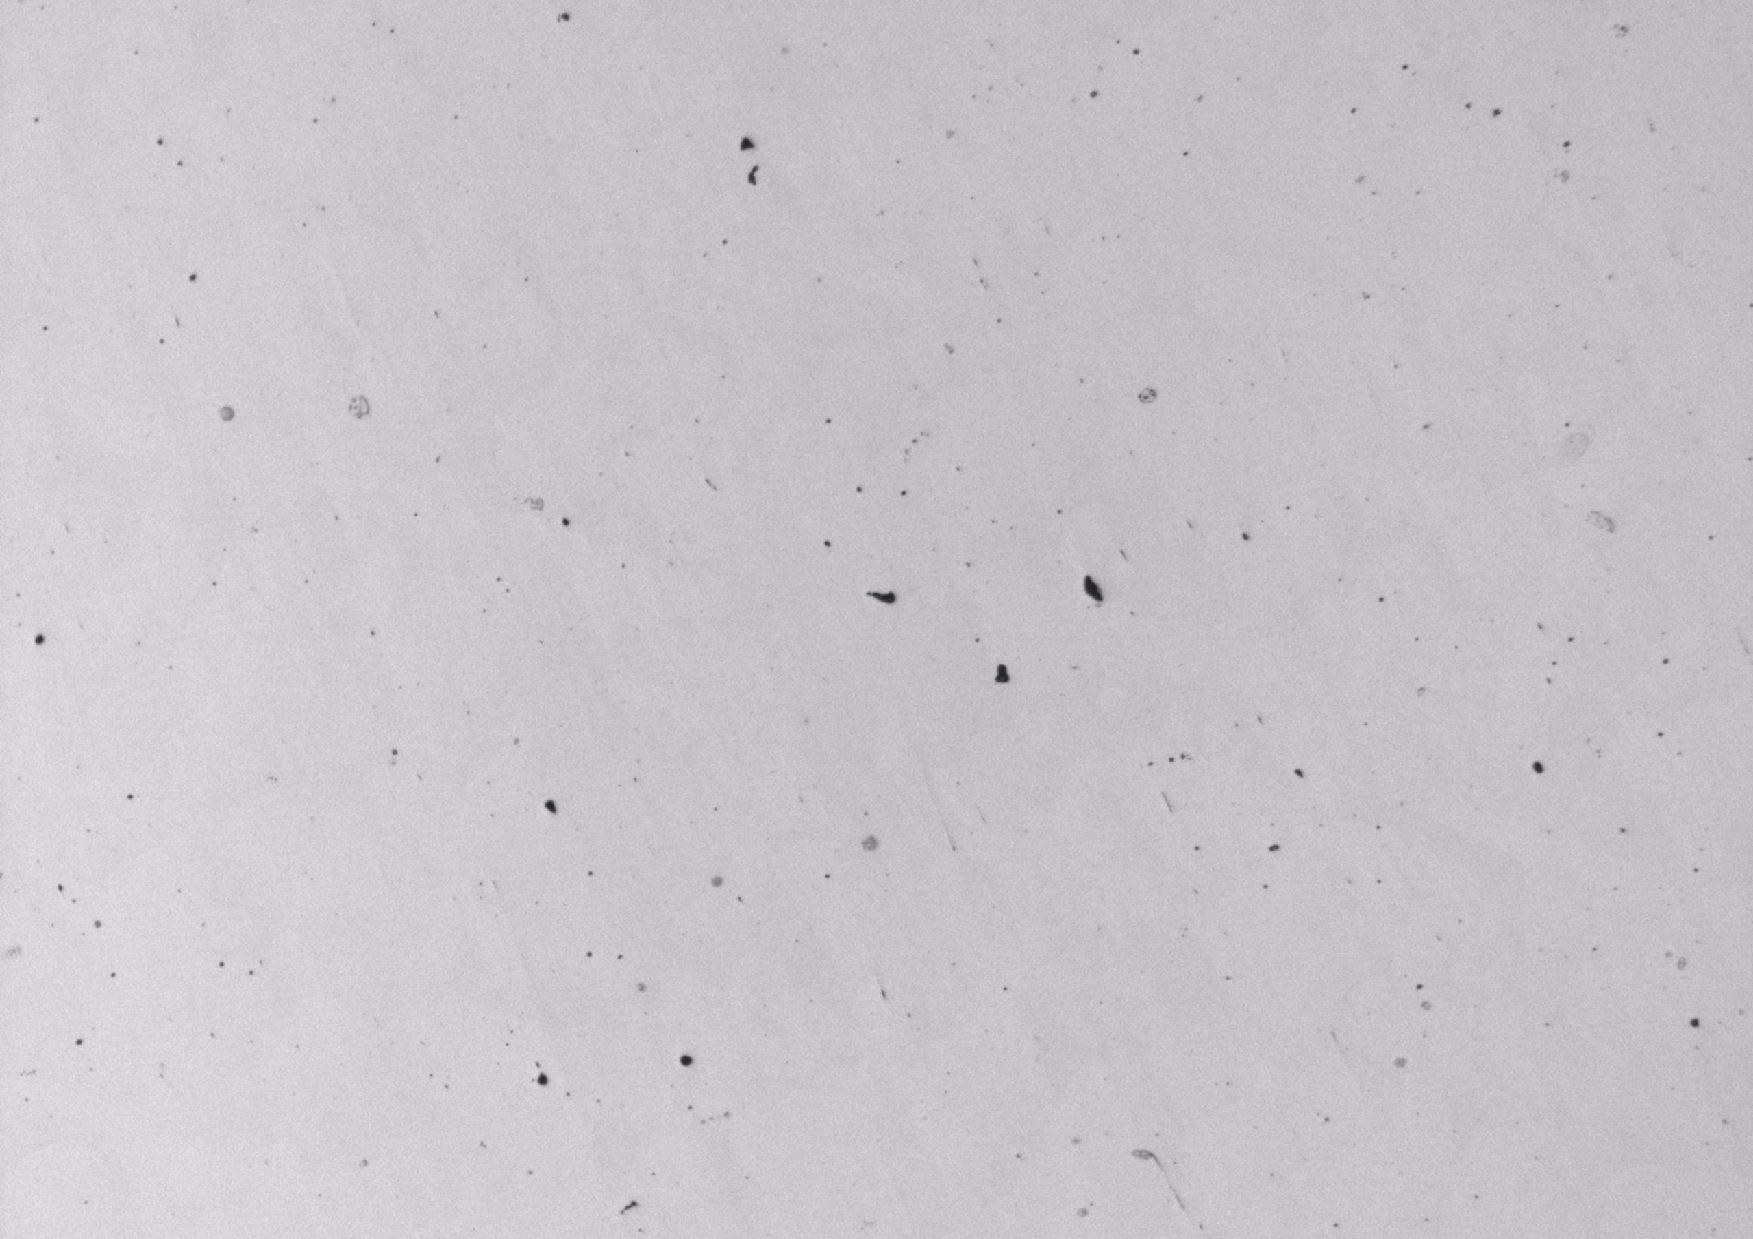
\includegraphics[width=0.75\textwidth]{images_optique/brut2.pdf}
    \caption{Echantillon brut de fonderie vu au microscope optique}
    \label{<label>}
\end{figure}

On mesure la proportion de défauts visibles au microscope optique à l'aide du 
logiciel d'analyse d'images ImageJ. Nous obtenons les résultats suivants : \\
\begin{table}
    \centering
    \caption{Proportion des différents défauts dans l'échantillon brut de fonderie}
    \begin{tabular}{c|c}
        \textbf{Type de défaut}  & \textbf{Proportion observée}  \\
        \hline
        Pore               & 0,340 \% \\
        Agrégat eutectique & 0,252 \% \\
    \end{tabular}

\end{table}

Nous voyons ainsi une proportion assez nette de défauts au sortir de la fonderie. 
Les agrégats eutectiques apparaissent pendant le refroidissement 
et la solidification du liquide. En effet, la vitesse de refroidissement dans 
la pièce est très difficile à contrôler précisément, et est donc nécessairement
inhomogène. Ainsi, certaines zones vont commencer à solidifier avant d'autres, et 
vont donc modifier la composition chimique du liquide qui les entoure. 

% \centerline{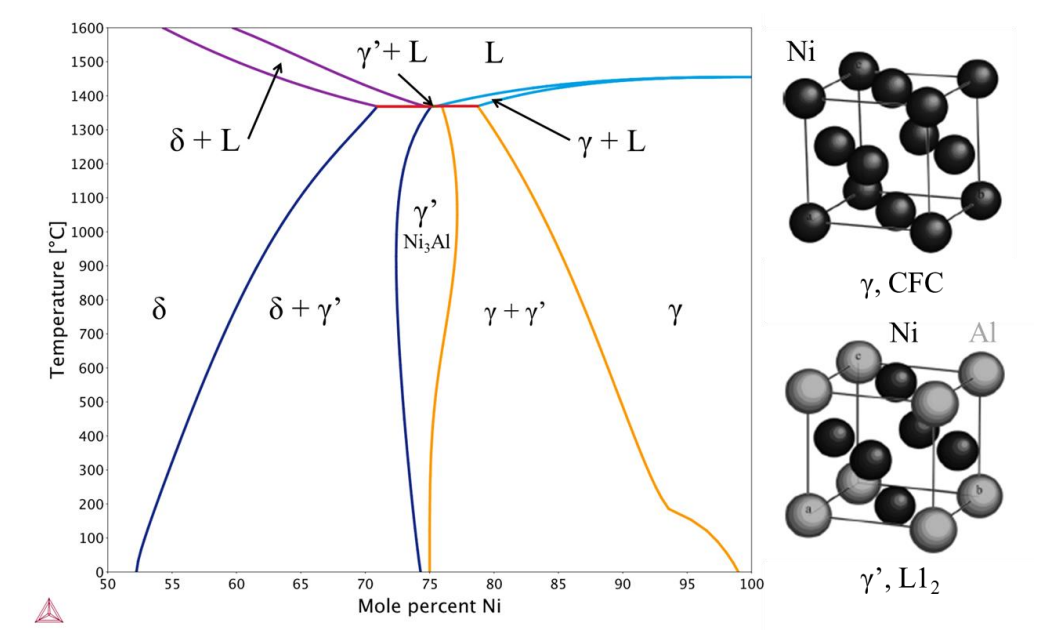
\includegraphics[width=0.75\textwidth]{images/diagramme_phase.png}}
% \legend{Diagramme Ni-Al avec les structures cristallines de la phase $\gamma$ et de la phase $\gamma'$}

\begin{figure}[htbp]
    \centering
    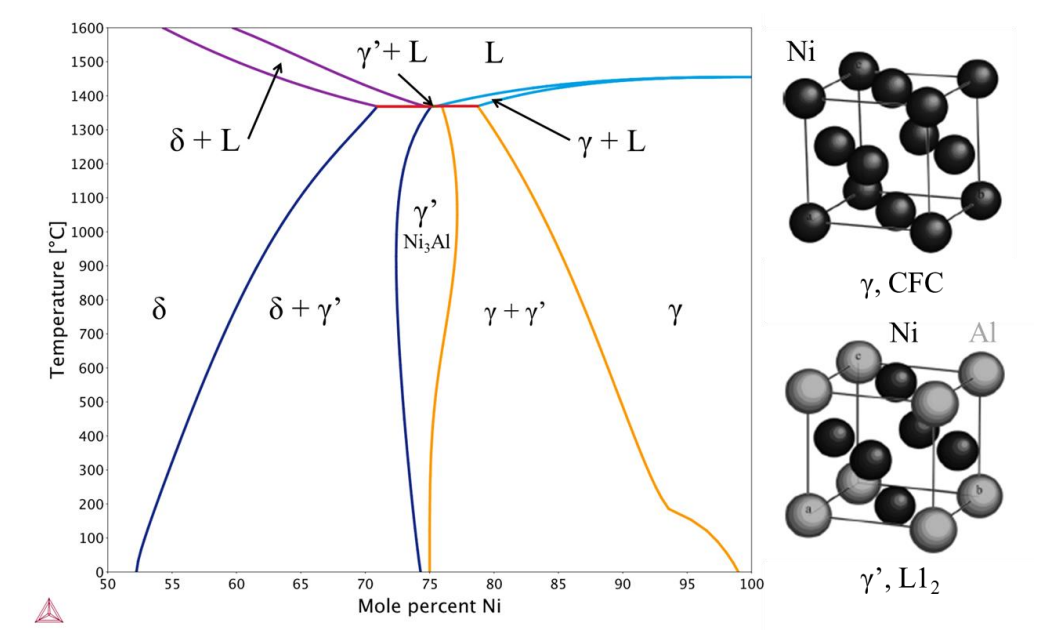
\includegraphics[width=0.75\textwidth]{images/diagramme_phase.png}
    \caption{Diagramme Ni-Al avec les structures cristallines des phases $\gamma$ et $\gamma'$}
    \label{<label>}
\end{figure}

% Quand on regarde le diagramme de phases nickel-aluminium, nous voyons que 
% lors de la solidification, le liquide va s'appauvrir en nickel et sa composition
% va tendre vers celle du liquide eutectique. Cela conduit donc à la formation de zones
% donc la composition est celle de l'assemblage $\gamma$/$\gamma'$, et d'autres zones 
% contenant uniquement la phase $\gamma'$ qui correspondent aux agrégats eutectiques.

De plus, les dendrites, qui sont les parties qui solidifient en premier, sont composées 
principalement de phase $\gamma$ (d'après le diagramme de phases nickel-aluminium), 
ce qui va modifier l'équilibre dans le liquide.
Les espaces inter-dendritiques vont ensuite se former,  plus riches en phase $\gamma'$, 
suivis enfin par les agrégats eutectiques composés de phase $\gamma'$.

Quant aux pores, leur apparition est liée à un flux trop faible de soluté 
dans les espaces inter-dendritiques, c'est-à-dire que la solidification de 
certaines zones se fait sans que le liquide ou la diffusion aient eu le 
temps de combler certains vides créés par la contraction du liquide qui
se refroidit. Nous avons donc un certain nombre de lacunes et de pores qui
apparaît ; ce nombre varie en fonction de la vitesse de refroidissement 
de la pièce.


\subsection*{Remis en solution}

Regardons maintenant notre échantillon après la remise en solution. 
Ce traitement consiste à réchauffer la pièce à très haute température (\SI{1300}{\celsius}),
mais en-dessous du point de fusion de l'alliage : aucun liquide n'est donc formé. 

Ce traitement a pour but d'homogénéiser la composition de l'alliage. En effet, nous avons 
vu différentes zones se solidifient à différents moments, ce qui place une partie de l'alliage
hors équilibre (comme par exemple les agrégats eutectiques). Le chauffage intense va également 
permettre d'accèlérer la diffusion dans l'alliage, et donc faciliter le mouvement des atomes 
(notamment les plus lourds comme le rhénium). 

Observons donc notre échantillon ayant subit une étape de remise en solution au microscope optique.

\begin{figure}[htbp]
    \centering
    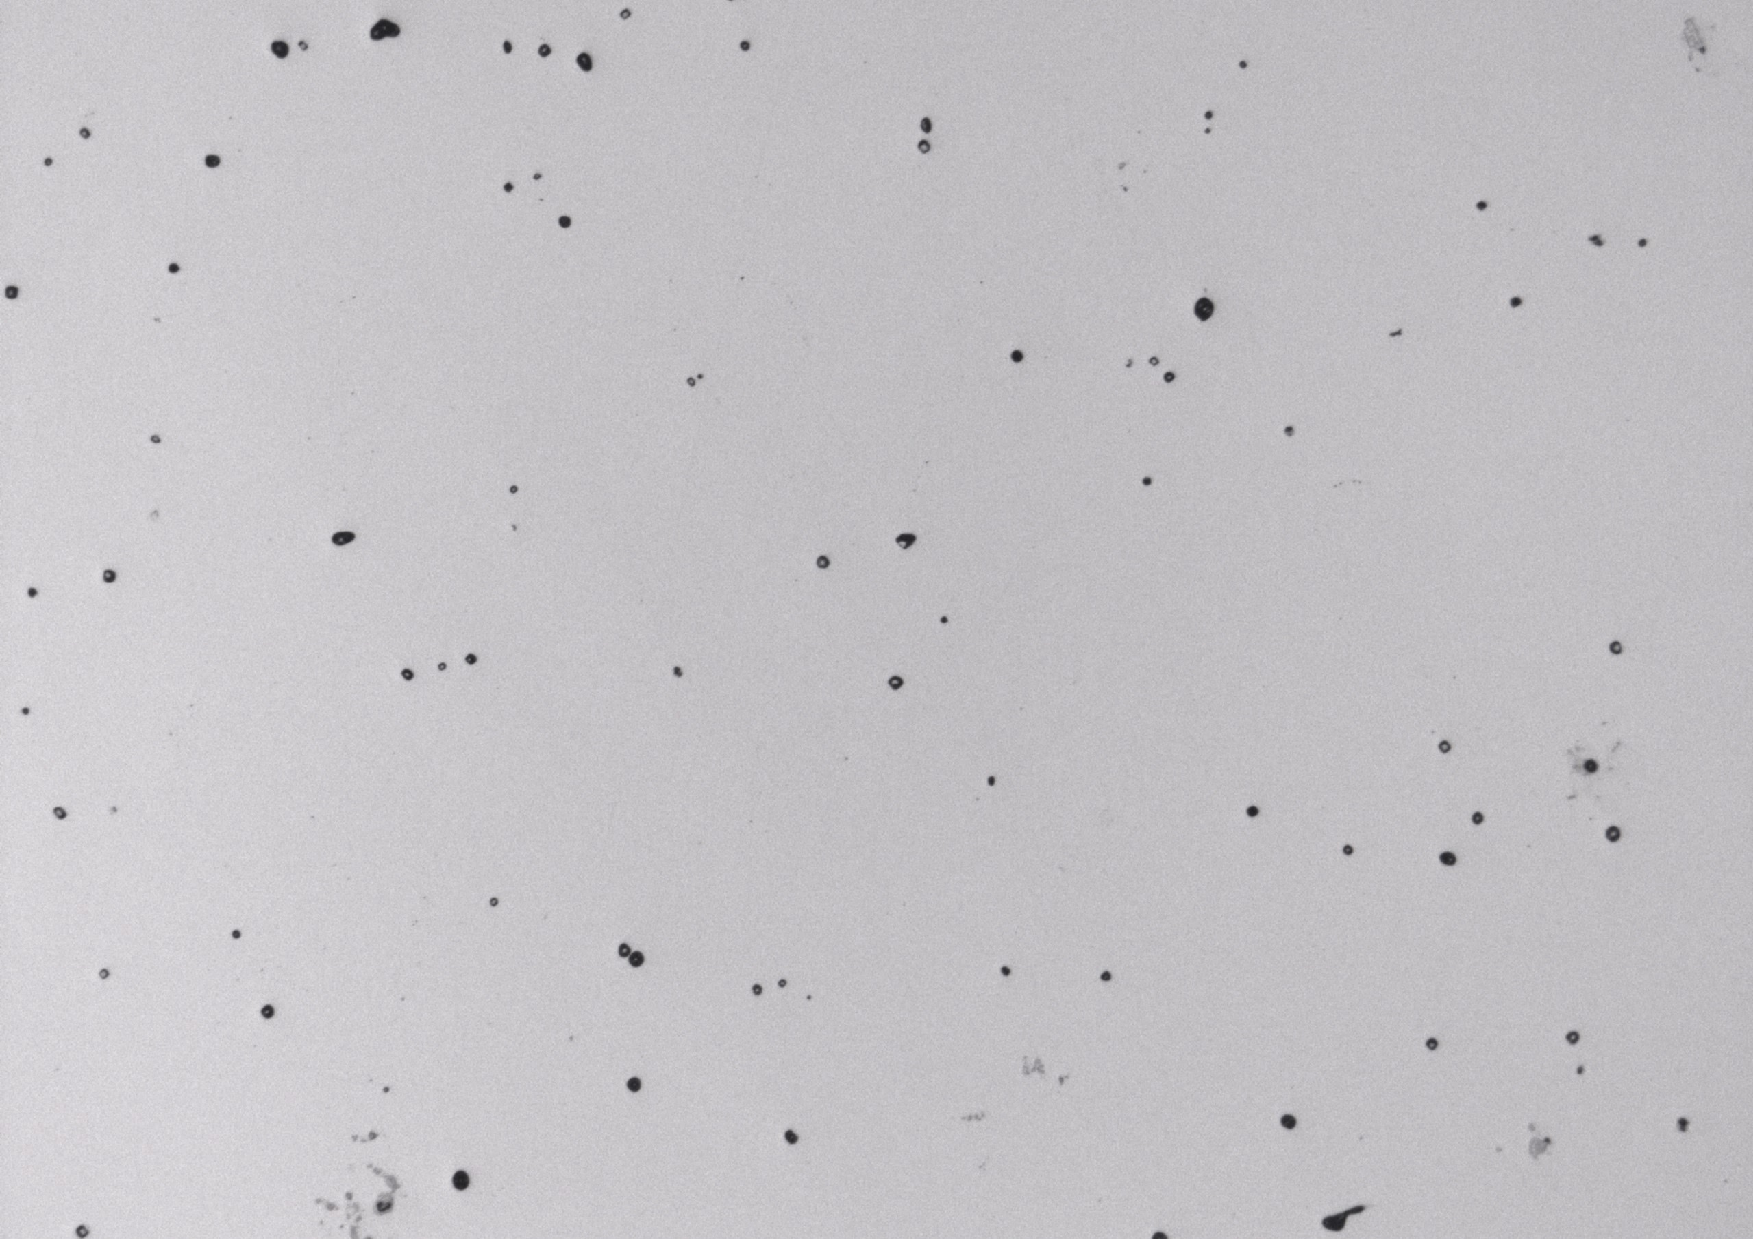
\includegraphics[width=0.55\textwidth]{images_optique/res.pdf}
    \caption{Echantillon après traitement de remise en solution}
    \label{<label>}
\end{figure}

Nous voyons que les agrégats eutectiques, très visibles sur le brut, ont quasiment disparu.
Ils étaient en effet nettement hors équilibre et donc peu stables thermodynamiquement. 

Néanmoins, nous avons augmenté le nombre de pores 

